\subsubsection{Activation function}\label{activationfunction}

The neural network explained until this point can be proved mathematically that the effect of adding up many linear regression operations is equivalent to a single linear regression. This is demonstrated in section \ref{feedforward}. The perception that has been created can collapse to the equivalent of having a single neuron. To avoid this, we need to calculate values that do not result in a linear function (a straight line in two dimensions), we need each of these neurons to apply some kind of non-linear manipulation that distorts their output values and for this we use the activation functions \cite{nielsen}.
\newline


As an example of the importance of activation functions, it will be shown with an example with a model with only linear functions compared to a model using non-linear functions. To do so, the following example is presented: we want to create a regression model that tries to predict the value of a sine function. Since the sine is a non-linear function, non-linear functions will be needed to solve the problem.

\begin{equation}
    y = \sin(x)
\end{equation}


Code will also be shown to introduce the operation of the libraries that are popularly used in the \acrlong{ml} world. As it is explained in section \ref{used_libs}, in this work \small{\verb|keras|}\normalsize (neural networks), \small{\verb|numpy|}\normalsize (vectors and matrices) and \small{\verb|matplotlib|}\normalsize (represent functions) among others have been used.
\newline

As explained in the training section (section \ref{training}), a dataset is needed for the network to be trained. The dataset will be created as follows:

\begin{minted}[fontsize=\footnotesize]{python}
# real sin data
x = np.linspace(0, 2*np.pi, 1000)
y = np.sin(x)

# some noise is added to the real dataset to make it 
# look like a real world data set
noise = 0.1
noisex = x + np.random.normal(-noise, noise, 1000)
noisey = y + np.random.normal(-noise, noise, 1000)
\end{minted}

Graphically a series of points would be scattered around the sine function as expected:
\begin{figure}[H]
    \centering
    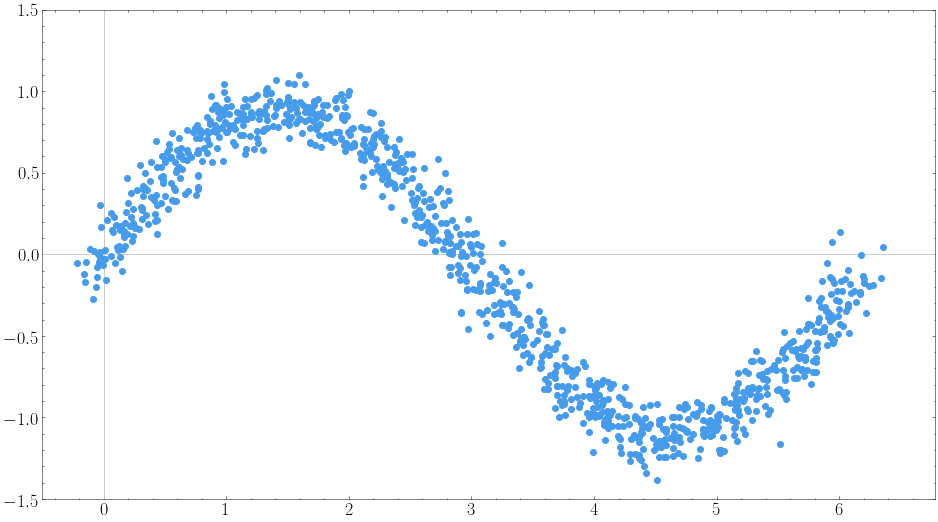
\includegraphics[width=11cm]{images/state-of-art/activation-functions/sin.png}
    \caption{Dataset emulating a sine function.}
    \label{fig:basicneuron}
\end{figure}

Two models will be created, i.e. two networks with different architectures: one model with linear activation functions (\small{\verb|linear_model|}\normalsize) and one with non-linear activation functions (\small{\verb|relu_model|}\normalsize).
\newline


The first model is defined as follows:

\begin{minted}[fontsize=\footnotesize]{python}
linear_model = Sequential()
linear_model.add(Dense(32, activation='linear'))
linear_model.add(Dense(32, activation='linear'))
linear_model.add(Dense(1))
\end{minted}

What is done in that code is to create the architecture of the network. It will be a network with three dense layers. The first two layers are the hidden layers of the model and it is indicated that 32 neurons are wanted in each layer with the \small{\verb|linear|} \normalsize  activation function. The last layer is simply so that the model only returns a single value.
\newline

The other network will use a non-linear \acrshort{relu} activation function, explained below.
The code for the architecture of this network is as follows:
\begin{minted}[fontsize=\footnotesize]{python}
relu_model = Sequential()
relu_model.add(Dense(32, activation='relu'))
relu_model.add(Dense(32, activation='relu'))
relu_model.add(Dense(1))
\end{minted}


The model is then compiled. In this step, Keras will be told that both mandatory and optional parameters are wanted for the network. These parameters will be explained in the next sections. Right after that the models are trained.
\begin{minted}[fontsize=\footnotesize]{python}
# Compile linear model
linear_model.compile(loss='mean_squared_error', 
                     optimizer='adam')
# Train linear model
linear_model.fit(noisex, noisey, epochs=100, verbose=0)

# Compile ReLU model
relu_model.compile(loss='mean_squared_error',
                   optimizer='adam')
# Train ReLU model
relu_model.fit(noisex, noisey, epochs=100, verbose=0)
\end{minted}

To study the models you can simply use the \small{\verb|predict()|} \normalsize function of the model:
\begin{minted}[fontsize=\footnotesize]{python}
predicted_by_linear = linear_model.predict(x)
predicted_by_relu = relu_model.predict(x)

# Plot predictions
plt.plot(x, predicted_by_linear)
plt.plot(x, predicted_by_relu)
\end{minted}

\begin{figure}[H]
    \centering
    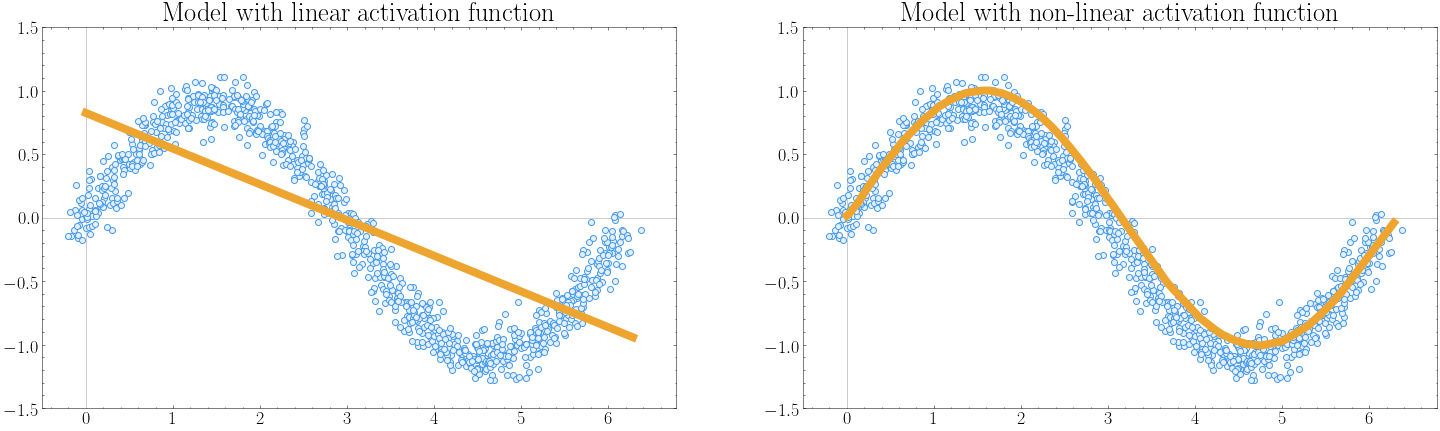
\includegraphics[width=15cm]{images/state-of-art/activation-functions/sin_activation_function.png}
    \caption{Comparison of linear and non-linear activation functions}
    \label{fig:basicneuron}
\end{figure}

As can be seen, the model using a linear trigger function is reduced to a single line while the model using a non-linear trigger function is adapted correctly.
\newline


In short, the trigger function is a function that applies to the result of the weighted sum of the input values, i.e., a $z$. The aim is that it distorts the result of the neuron by adding non-linear deformations to it so that the computation of several neurons can be effectively linked. This activation function will be represented as follows:

\begin{equation}
    a(z) = a(w \cdot x + b)
    \label{eqn:activationfunctionbasic}
\end{equation}

By updating the image that has been used before to define a perception, it would look like this:
\begin{figure}[H]
    \centering
    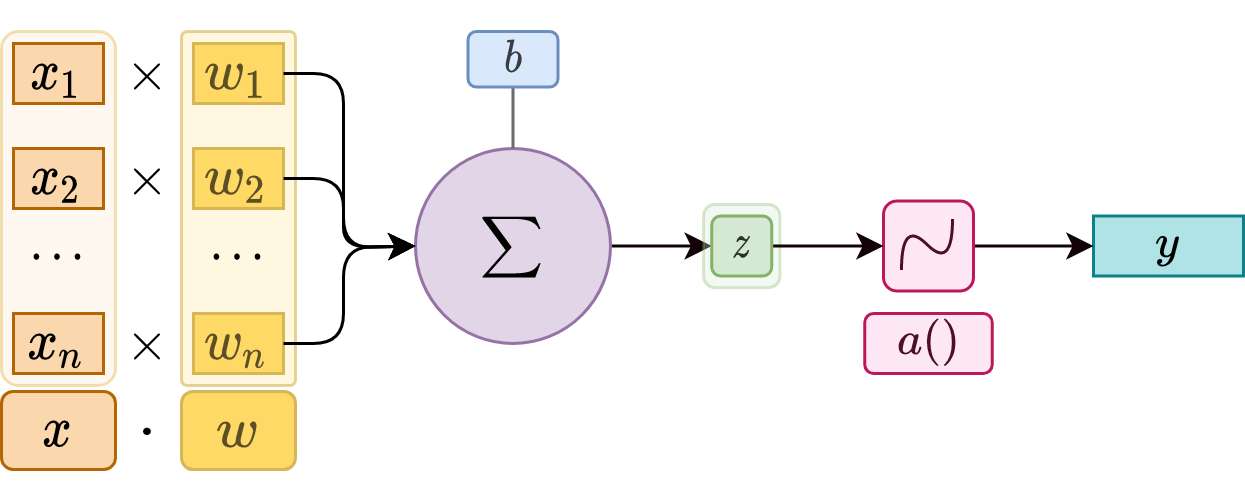
\includegraphics[width=10cm]{images/state-of-art/activation-functions/activation_representation.png}
    \caption{Representation of how a neuron works.}
    \label{fig:basicneuron}
\end{figure}

There are several types of activation function, these are the most used:

\begin{itemize}
\item Linear: It is simply the equation of a line and therefore a linear function. It is usually used in the last layer in a regression model, that is, a model that performs a regression task and not a classification task.
\begin{eqnarray}
  a(z) & = & z \\
  a'(z) & = & 1 
\end{eqnarray}

\item Step: The objective of the function is to convert the values to $0$ or $1$ as a function of $b$. The purpose of this activation function is to imitate a neuron that "activates" or "does not activate" based on the input information. Traditionally, this function was used in networks of perceptrons and in fact, it is the one used in equation \ref{eqn:perceptroncomplex}:


\begin{eqnarray}
  a(z) & = & \left\{ \begin{array}{ll}
      0 & \mbox{si } z \leq 0 \\
      1 & \mbox{si } z > 0
      \end{array} \right. \\
     \newline
  a'(z) & = & 0 
\end{eqnarray}


\item \acrlong{relu}: It is a linear function when it is positive and constant at 0 when the value is negative. It is widely used because it is a non-linear function and similar to the linear function, so it is fast to compute.

\begin{eqnarray}
    a(z) & = & max(0,z) \\
  a'(z) & = & \left\{ \begin{array}{ll}
      0 & \mbox{si } z \leq 0   \\
      1 & \mbox{si } z > 0 
      \end{array} \right.
\end{eqnarray}

There is a variant of this activation function (known as leaky). In this variant, the slope is changed to a value $s$ of the negative part with respect to the abscissa axis.

\begin{eqnarray}
    a(z) & = & \left\{ \begin{array}{ll}
      s & \mbox{si } sz \leq 0   \\
      z & \mbox{si } z > 0 
      \end{array} \right. \\
  a'(z) & = & \left\{ \begin{array}{ll}
      s & \mbox{si } sz \leq 0   \\
      1 & \mbox{si } z > 0 
      \end{array} \right.
\end{eqnarray}


\item Sigmoid ($\sigma$): This is the most commonly used function in neural networks. The distortion it produces to very large values make them saturated at $1$ and very small values makes them saturated at $0$. This function is very useful to represent probabilities since they always come in the range of $[0, 1]$ and as explained in section \ref{models}, probability is the perfect tool for \acrlong{ml}. Moreover, this function, together with $tanh$, achieves a fluidity that is not achieved with the functions explained above. A small change in $w$ or $b$ will produce a small change in the output value.

\begin{eqnarray}
    a(z) & = & \frac{\mathrm{1} }{\mathrm{1} + e^{-z} } \\
    a'(z) & = & a(z) (1 - a(z))
\end{eqnarray}

\item Hyperbolic tangent ($tanh$): This is similar to the sigmoid, but the range of output values is $[-1,1]$.
\begin{eqnarray}
    a(z) & = & tanh(z) \\
    a'(z) & = & 1 - tanh(z)^2
\end{eqnarray}


\end{itemize}

Each of the functions explained in graphic form is shown below:
\begin{figure}[H]
    \centering
    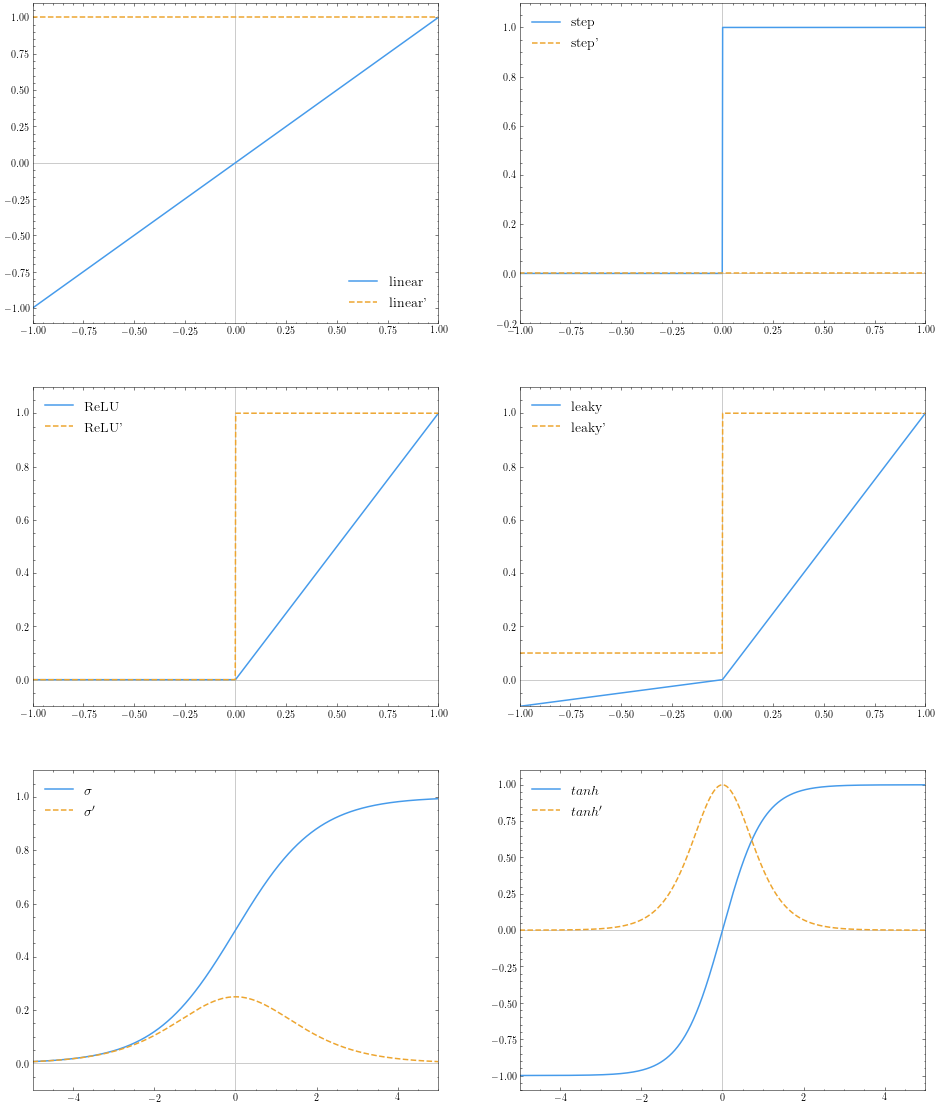
\includegraphics[width=15cm]{images/state-of-art/activation-functions/activation_functions.png}
    \caption{Graphs of the activation functions.}
    \label{fig:basicneuron}
\end{figure}

Each neuron may have an associated activation function, but by convention only one type of activation function is used for each layer. Both solutions give similar results and neither brings in principle significant improvements to the outcome of the model. The main difference is the added complexity of developing a network if a different activation function is to be used per neuron. In conclusion, the use of a single activation function on all the neurons in a layer is always chosen for simplicity of development.
\newline